% formato document
\documentclass[12pt,a4paper,openright,twoside]{report}
% import pacchetti lingua e enconding
\usepackage[english,italian]{babel}
\usepackage{lmodern}
\usepackage[T1]{fontenc}
\usepackage[utf8]{inputenc}
% code highlighting
\usepackage{algorithm}
\usepackage[noend]{algpseudocode}
\algrenewcommand\algorithmicindent{1.0em}
%%%%
\usepackage{listings}
\usepackage{minted}
\definecolor{bg}{rgb}{.9,.9,.95}
\usemintedstyle{trac}
% utilit
\usepackage{afterpage}
% modifica numbering sezioni
\usepackage{titlesec}
%\renewcommand{\thesubsection}{}
%\setcounter{secnumdepth}{2}
% pacchetti ams
\usepackage{amsmath}
\usepackage{amsfonts}
\usepackage{amssymb}
\usepackage{amsthm}
\newtheorem{definition}{Definizione}
\newtheorem{lemma}{Lemma}
% esempi
\theoremstyle{definition}
%\newtheorem{example}{Esempio}[section]
\newcounter{examp} 
\setcounter{examp}{1}
\newenvironment{example}[0]{\textbf{Esempio \arabic{examp}}}{\refstepcounter{examp}}
% pacchetto tikz per disegnare i grafi
\usepackage{subfig}
\usepackage{caption}
%\usepackage{subcaption}
\usepackage{empheq}
\usepackage{tikz}
\usetikzlibrary{arrows}
%renew captions
%\renewcommand{\figurename}{Esempio}
\usepackage[labelfont=bf,justification=justified,font=small,font+=it]{caption}
%alberi
\tikzset{
  treenode/.style = {align=center, text centered,
    font=\sffamily},
  arn_n/.style = {treenode, circle, black, font=\sffamily\bfseries, draw=black,
    fill=white},% arbre rouge noir, noeud noir
}
%immaginiiiiiii
\usepackage{graphicx}
%%%%%%%%%%%%%%%%%%
%INIZIO DOCUMENTO%
%%%%%%%%%%%%%%%%%%

\begin{document}
\begin{titlepage}
\title{"XML Covering Index utilizzando la relazione di Simulazione}
\date{\today}
\author{Luca Casini\\Università degli studi di Perugia\\Corso di Laurea in Informatica}
\end{titlepage}
\maketitle
\tableofcontents

%\mainmatter
%\pagestyle{headings}

%%%%%%%%%%%%%%%%%%%%%%%%%%%%%%%%%%%%
%CAPITOLO 1 - NOZIONI INTRODUTTIVE %
%%%%%%%%%%%%%%%%%%%%%%%%%%%%%%%%%%%%

\chapter{Nozioni Introduttive}
Iniziamo introducendo alcune nozioni alla base di questa tesi: i \textbf{grafi}, strutture matematiche utilizzate nella rappresentazione dei documenti XML, e le relazioni di \textbf{Simulazione}, \textbf{Bisimulazione} e \textbf{Trace Equivalence}, relazioni binarie sui grafi che possono essere usate nella creazione di indici XML.

\section{I Grafi}
Introduciamo formalmente il concetto di grafo e le notazioni che utilizzeremo nel corso della tesi.
\\\\
I grafi sono strutture matematiche di grande importanza in molteplici campi scientifici. Un grafo è composto da un insieme di entità astratte chiamate \textbf{nodi} e un insieme di coppie di nodi, detti \textbf{archi}, che sono in relazione tra loro.\\
Possiamo rappresentare graficamente un grafo come dei punti nello spazio, i nodi, connessi da delle linee, gli archi.

\begin{definition}[Grafo]
E' chiamato Grafo una coppia di insiemi $G = (N,E)$ dove $N$ è un insieme non vuoto di elementi detti nodi e $E \in N \times N $ è l'insieme degli elementi detti archi. Chiameremo $|N\,|$ \textbf{ordine} del grafo e $|E\,|$ \textbf{dimensione} del grafo.
\end{definition}

Se esiste in $E$ un insieme di archi che ci permette di raggiungere un nodo $v$ partendo da un altro nodo $u$ diremo che esiste un cammino tra i due nodi.

\begin{definition}[Cammino]
dati due nodi $u,v \in N$ esisterà un cammino $u ~ v$ di lunghezza $k$ se esiste una sequenza $<v_0,v_1,v_2,...,v_k>$ di vertici tale che la coppia $(v_(i-1),v_i) \in E$ per $i = 1,..,k$, con $u = v_0$ e $v = v_k$. 
\end{definition}

In base alle proprietà che verificano possiamo dividere i grafi nel seguente modo:

\begin{itemize}
\item un grafo può essere \textbf{finito o infinto} a seconda della cardinalità di $N$.
\item un grafo si dice \textbf{etichettato} se ad ogni nodo e/o vertice è associata una etichetta di qualche tipo.
\item un grafo è \textbf{aciclico} se e soltanto se non esiste un cammino che riporti al nodo di partenza, ossia $\not\exists u \in N: <u,u> \in E$.
\item un grafo è detto \textbf{orientato} nel caso in cui gli archi abbiano un verso di percorrenza; un grafo semplice è non orientato ovvero $(u,v)\in E \implies (v,u) \in E$.
\end{itemize}

%\textcolor{red}{DEFINIZIONE DI COMPONENTI CONNESSE FORSE NON NECESSARIA?}

\begin{definition}[Grafo fortemente connesso]
Un grafo orientato è \textbf{fortemente connesso} se due vertici qualsiasi sono raggiungibili l'uno dall'altro, ovvero per ogni $ u, v \in \: N $, vale $ u \: \leadsto \: v $.
\end{definition}

\begin{definition}[Componente fortemente connessa]
Una \textbf{componente fortemente connessa} di un grafo orientato $G$ è un sottografo massimale di $G$ fortemente connesso in cui esiste un cammino orientato tra ogni coppia di nodi ad esso appartenenti.
\end{definition}
Le componenti fortemente connesse formano una partizione di $G$ poiché un nodo non può trovarsi contemporaneamente in due componenti fortemente connesse, di conseguenza un grafo orientato è fortemente connesso se e solo se ha una sola componente connessa
In seguito illustriamo alcuni esempi con i vari tipi di grafi:\\\\
\begin{example} 
\begin{figure}[H]
\subfloat[Grafo ciclico non orientato]{
\begin{tikzpicture}[>=stealth',shorten >=1pt,scale=.4,node distance=2cm,
  thick,main node/.style={circle,fill=white,draw,font=\sffamily\Large\bfseries}]
  
   \node[main node] (1) {1};
  \node[main node] (2)[below right of=1] {2};
  \node[main node] (5) [right of=2]{5};
  \node[main node] (3) [below  of=2] {3};
  \node[main node] (4) [right of=3] {4};
  \node[main node] (6) [below right  of=5] {6};	  


  \path[every node/.style={font=\sffamily\small}] 
         (1) edge node [] {} (2)	  
  		 (2) edge node [] {} (3)
  		 	edge node [] {} (5)
  		 (3) edge node [] {} (4) 			
  		 (4) edge node [] {} (5)
  		 edge node [] {} (6)
  		 (5) edge node [] {} (6);
\end{tikzpicture}}
\qquad
\subfloat[Grafo aciclico non orientato]{
\begin{tikzpicture}[>=stealth',shorten >=1pt,scale=.4,node distance=2cm,
  thick,main node/.style={circle,fill=white,draw,font=\sffamily\Large\bfseries}]

 %\tikzset{ container/.style={draw , ellipse , dashed , inner sep =0.1em}}
  
  \node[main node] (1) {1};
  \node[main node] (5) [right of=1] {5};
  \node[main node] (4) [below left of=5]{4};
  \node[main node] (2) [below left of=1] {2};
  \node[main node] (6) [below right of=4] {6};
  \node[main node] (3) [below  of=2] {3};	  

%\node[container , fit=(2) (4)] (b1) {};
%\node at (b1.west) [left ,node distance=2 and 1] {B2: };
  \path[every node/.style={font=\sffamily\small}] 
         (1) edge node [] {} (2)	  
  		 (2) edge node [] {} (4)
  		 	edge node [] {} (3)
  		 (4) edge node [] {} (5)
  		 	edge node [] {} (6);
\end{tikzpicture}}
\caption{Grafi ciclici/aciclici non orientati etichettati sui nodi\label{fig:1}}
\end{figure}
\end{example}

\begin{example}

\begin{figure}[H]

\centering%

\subfloat[Grafo ciclico orientato che contiene il ciclo \{1,2,4,1\}]
{
\begin{tikzpicture}[->,>=stealth',shorten >=1pt,auto,node distance=2cm,
  thick,main node/.style={circle,fill=white,draw,font=\sffamily\Large\bfseries}]
  
  \node[main node] (1) {1};
  \node[main node] (2) [below left of=1] {2};
  \node[main node] (3) [below right of=1] {3};
  \node[main node] (4) [below right of=2] {4};
  
  \path[every node/.style={font=\sffamily\small}] 
         (1) edge node [] {} (2)
         	 edge node [] {} (3)
         		  
  		 (2) edge node [] {} (3)
  		 	 edge node [] {} (4)
  		 (4) edge node [] {} (1);
  
 \end{tikzpicture}

}
% 
\qquad
\subfloat[Grafo aciclico orientato]
{
   \begin{tikzpicture}[->,>=stealth',shorten >=1pt,auto,node distance=2cm,
  thick,main node/.style={circle,fill=white,draw,font=\sffamily\Large\bfseries}]
  
  \node[main node] (1) {1};
  \node[main node] (2) [below left of=1] {2};
  \node[main node] (3) [below right of=1] {3};
  \node[main node] (4) [below right of=2] {4};
  
  \path[every node/.style={font=\sffamily\small}] 
         (1) edge node [] {} (2)
         	 edge node [] {} (3)
         	 edge node [] {} (4)	  
  		 (2) edge node [] {} (3)
  		 	 edge node [] {} (4);
 \end{tikzpicture}
}
%
\caption{Grafi ciclici/aciclici orientati etichetatti sui nodi\label{fig:2}}

\end{figure} 
\end{example}

\begin{example}

\begin{figure}[H]
  \centering
   \begin{tikzpicture}[->,>=stealth',shorten >=1pt,auto,node distance=2cm,
  thick,main node/.style={circle,fill=white,draw,font=\sffamily\Large\bfseries}]
  
  \node[main node] (1) {1};
  \node[main node] (2) [below left of=1] {2};
  \node[main node] (3) [below right of=2] {3};
  \node[main node] (4) [right of=1] {4};
  \node[main node] (6) [below right of=4] {6};
  \node[main node] (5) [below left of=6] {5};
  
  \path[every node/.style={font=\sffamily\small}] 
         (1) edge node [] {} (3)
         	 edge node [] {} (4)	  
  		 (2) edge node [] {} (1)
  		 (3) edge node [] {} (2)	
  		 (4) edge node [] {} (5)
  		 (5) edge node [] {} (6)
  		 (6) edge node [] {} (4);
  
 \end{tikzpicture}
\caption{Un grafo orientato con due componenti fortemente connesse \{1,2,3\} e \{4,5,6\} \label{fig:3}}
\end{figure}
\end{example}

\newpage
\subsection{Alberi}
Questa tesi si occuperà di un tipo particolare di grafo detto \textbf{albero}. Un albero è un grafo aciclico che verifica certe proprietà; questo nome deriva dal fatto che, come un vero albero, possiede una radice da cui partono delle ramificazioni (sotto-alberi).
\begin{definition}[Albero]
Si dice albero un grafo $G$ che verifica una della seguenti condizioni equivalenti:
\begin{itemize}
\item $G$ è aciclico e connesso.
\item aggiungere un arco a $G$ crea un ciclo.
\item se si rimuovere un arco $G$ non è più connesso.
\end{itemize}
\end{definition}

La struttura dati comunemente utilizzata in informatica è una tipologia di albero detto radicato \emph{radicato}, cioè un albero in cui un nodo viene scelto come radice.

\begin{definition}
Definiamo di seguito la radice e tutti i componenti dell'albero a partire da essa:\\
\begin{description}
\item[Radice:] La radice è il nodo di partenza. Tra la radice e qualsiasi nodo dell'albero c'è un percorso univoco (il senso del percorso è dato dall'orientamento dell'albero, generalmente è dalla radice al nodo).
\item[Livello:] Il livello è dato dalla lunghezza del percorso dal nodo alla radice, la radice ha livello 0. Il livello massimo raggiunto è detto \textbf{altezza} dell'albero. I nodi allo stesso livello sono detti \textbf{cugini}.
\item[Discendente/Antenato:] Dato un nodo i suoi discendenti sono tutti i nodi da esso raggiungibili allontanandosi dalla radice. Muovendoci verso la radice troveremo i suoi Antenati.
\item[Figlio/Padre:] Dato un nodo i suoi figli sono i discendenti al livello inferiore. Il padre di un nodo è l'antenato al livello superiore. I nodi figli dello stesso padre si dicono \textbf{fratelli}.
\item[Foglia:] Un nodo è una foglia se non ha figli. E,->,>=' anche detto \textbf{nodo esterno}.
\end{description}
\end{definition}
%esempio albero
\begin{example}
\begin{figure}[H]
\centering
\begin{tikzpicture}[->,>=stealth',level/.style={sibling distance = 5cm/#1,
  level distance = 1.5cm}] 
\node [arn_n] {1}
    child{ node [arn_n] {2} 
            child{ node [arn_n] {4} 
            	child{ node [arn_n] {8}}							
            }
            child{ node [arn_n] {5}
							child{ node [arn_n] {9}}
            }                            
    }
    child{ node [arn_n] {3}
            child{ node [arn_n] {6} 
							child{ node [arn_n] {10}}
							child{ node [arn_n] {11}}
            }
            child{ node [arn_n] {7}
							child{ node [arn_n] {12}}
            }
		}
; 
\end{tikzpicture}
\caption{Esempio di Albero}\label{fig:albero}
\end{figure}
Nella figura \ref{fig:albero} vediamo un esempio di albero. Il nodo 1 è la radice, i nodi 8,9,10,11,12 sono foglie al livello 3. Il nodo 3 è padre del nodo 6 e 7 e antenato di 6,7,10,11,12. 
\end{example}


\section{Simulazione, Bisimulazione e Trace Equivalence}
In questa sezione introduciamo la relazione d'equivalenza detta simulazione e due relazione ad essa collegate: la bisimulazione e la trace equivalence.
\\\\
Le classi di equivalenza che costruiamo grazie a queste relazioni possono essere utilizzate per creare un grafo ridotto detto \textbf{grafo quoziente.}
L'uso del grafo quoziente permette, a fronte di una perdita di informazione, di lavorare con strutture più piccole risparmiando tempo e risorse.

\subsection{Simulazione}
Iniziamo definendo formalmente la relazione di simulazione, in seguito illustreremo un esempio su un albero.

\begin{definition}
Sia $G = (V, E,A, \langle\langle.\rangle\rangle)$ un grafo etichettato dove: 
\begin{itemize}
\item $V$ è l'insieme dei vertici.
\item $E \subseteq V^2$ è l'insieme dei cammini.
\item $A$ è l'insieme delle etichette.
\item $\langle\langle.\rangle\rangle:V \to A$ è una funzione che assegna ad ogni vertice $v$ la propria etichetta $\langle\langle v\rangle\rangle$.
\end{itemize}
Data la funzione $post(v) = \{u|(v,u) \in E\}$ che restituisce l'insieme dei successori del vertice $v$.
Possiamo definire una relazione binaria $\preceq\;\subseteq V^2$ detta \emph{simulazione} se si verificano le seguenti condizioni:
\begin{enumerate}
\item $\langle\langle u \rangle\rangle = \langle\langle v \rangle\rangle$
\item $\forall u' \in post(u) \exists v' \in post(v) | u' \preceq v'$
\end{enumerate}
\begin{lemma}
Due vertici $u$ e $v$ si dicono simili $u\approx^Sv$ se $u \preceq v$ e $v \preceq u$; la \emph{similarità} $\approx^S$ è una relazione di equivalenza.
\end{lemma}
\end{definition}
\begin{flushleft}
%figura simulazione
\begin{example}
\begin{figure}[H]
\centering
\subfloat[Grafo G]{
\begin{tikzpicture}[->,>=stealth',shorten >=1pt,auto,node distance=2cm,
                    thick,main node/.style={circle,draw,font=\sffamily\Large\bfseries}]

  %\node[main node] (1) {/};
  \node[main node] (2) [%below of=1,
  label=right:5] {a};
  \node[main node] (3) [below left of=2,label=right:4] {b};
  \node[main node] (4) [below right of=2,label=right:6] {b};
  \node[main node] (5) [below of=4,label=right:7] {c};
  \node[main node] (6) [below of=5,label=right:8] {d};  
  \node[main node] (7) [below of=3,label=right:3] {c};
  \node[main node] (8) [below left of=3,label=right:1]{c};  
  \node[main node] (9) [below of=7,label=right:2]{d};
  
  \path[every node/.style={font=\sffamily\small}]
   % (1) edge node {} (2)
    (2) edge node {} (3)
        edge node {} (4)
    (3) edge node {} (7)
        edge node {} (8) 
    (4) edge node {} (5)
    (5) edge node {} (6)
    (7) edge node {} (9)
    (9) edge [loop left] node {} (9)
    (6) edge [loop left] node {} (6);
\end{tikzpicture}}
\qquad
\subfloat[Grafo $G/_{\simeq^S}$]{
\begin{tikzpicture}[scale=1,->,>=stealth',shorten >=1pt,auto,node distance=2cm,
                    thick,main node/.style={scale=1,circle,draw,font=\sffamily\Large\bfseries}]

  %\node[main node] (1) {/};
  \node[main node] (2) [%below of=1,
  label=right:5] {a};
  \node[main node] (3) [below of=2,label=right:4 6] {b};
  \node[main node] (4) [below left of=3,label=right:1] {c};
  \node[main node] (5) [below right of=3,label=right:3 7] {c};
  \node[main node] (6) [below of=5,label=right:2 8] {d};

  \path[every node/.style={font=\sffamily\small}]
    %(1) edge node {} (2)
    (2) edge node {} (3)
    (3) edge node {} (4)
        edge node {} (5) 
    (5) edge node {} (6)
    (6) edge [loop left] node {} (6);
\end{tikzpicture}}
\caption{Esempio di Simulazione.\label{fig:simulaizone}}
\end{figure}
A sinistra abbiamo il grafo di partenza e a destra il grafo quoziente ricavato dalla relazione $\simeq^S$. Da notare come la cardinalità sia quasi dimezzata nel grafo quoziente.
\end{example}
\end{flushleft}
\subsection{Bisimulazione}
Definiamo ora la relazione di bisimulazione
\begin{definition}
Dati due vertici $u$ e $v$, $u \simeq v$ se:
\begin{itemize}
\item $\langle\langle u \rangle\rangle = \langle\langle v \rangle\rangle$
\item $\forall u' \in post(u) \exists v' \in post(v) | u' \simeq v'$
\item $\forall v' \in post(v) \exists u' \in post(u) | v' \simeq u'$
\end{itemize}
Diremo quindi che $u$ bisimula $v$; se $u \simeq v$ e $v \simeq u$ allora si ha una relazione di \emph{bisimulazione} $\approx^B$.
\end{definition}
Il grafo quoziente $G/_{\approx^B}$ conserva un linguaggio più espressivo rispetto a quello ottenuto sfruttando la simulazione ma, essendo una relazione più fine, non fornisce una riduzione altrettanto importante in termini di spazio. Va notato come grazie all'algoritmo di Paige-Tarjan è possibile calcolare la bisimulazione in $O(mlogn)$.


\subsection{Trace Equivalence}
Illustriamo infine la trace equivalence, in figura possiamo vedere un confronto tra le due relazioni.
\begin{definition}
Dati due vertici $u$ e $v$, diciamo che $u$ domina $v$ se:
\begin{itemize}
\item definito $\bar{u}$ un cammino con radice in $u$
\item $\forall\,\bar{u}\quad\exists\,\bar{v}\;|\;\langle\langle \bar{u} \rangle\rangle\,=\, \langle\langle \bar{v} \rangle\rangle$
\end{itemize}TraceG
La relazione di equivalenza $\approx^T$ è detta Trace Equivalence e vale se $u$ domina $v$ e $v$ domina $u$.
\end{definition}
\begin{lemma}
La trace equivalence è implicata dalla simulazione ma non viceversa.
\end{lemma}
Questa relazione è molto importante perché due vertici equivalenti soddisfano le stesse formule di LTL e quindi il grafo quoziente $G/_{\approx^T}$ può essere usato per verificarle; tuttavia costituire questo grafo è molto difficile, il problema infatti è PSPACE-completo.\\\\
\newpage
\begin{example}
\begin{figure}[H]
\centering
\subfloat[Grafo G]{
\begin{tikzpicture}[->,>=stealth',shorten >=1pt,auto,node distance=2cm,
                    thick,main node/.style={circle,draw,font=\sffamily\Large\bfseries}]

\node[main node] (1) [label=right:1] {r};
\node[main node] (2) [below left of=1,label=right:2] {a};
\node[main node] (3) [below right of=1,label=right:3] {a};
\node[main node] (4) [below of=2,label=right:4] {b};
\node[main node] (5) [below right of=2,label=right:5] {b};
\node[main node] (6) [below of=3,label=right:6] {b};
\node[main node] (7) [below of=4,label=right:7] {c};
\node[main node] (8) [below of=5,label=right:8] {c};
\node[main node] (9) [below of=6,label=right:9] {d};

\path[every node/.style={font=\sffamily\small}]
(1) edge node {} (2)
    edge node {} (3)
(2) edge node {} (4) edge node {} (5)
(3) edge node {} (6) edge node {} (5)
(4) edge node {} (7)
(5) edge node {} (8)
(6) edge node {} (9)    
(7) edge [loop left] node {} (7)
(8) edge [loop left] node {} (8)
(9) edge [loop left] node {} (9);
\end{tikzpicture}
}
\subfloat[Grafo $G/_{\approx^B}$]{
\begin{tikzpicture}[->,>=stealth',shorten >=1pt,auto,node distance=2cm,
                    thick,main node/.style={circle,draw,font=\sffamily\Large\bfseries}]

\node[main node] (1) [label=right:1] {r};
\node[main node] (2) [below left of=1,label=right:2] {a};
\node[main node] (3) [below right of=1,label=right:3] {a};
%\node[main node] (4) [below left of=2,label=right:4] {b};
\node[main node] (5) [below right of=2,label=right:4-5] {b};
\node[main node] (6) [below of=3,label=right:7-8] {b};
%\node[main node] (7) [below of=4,label=right:4] {c};
\node[main node] (8) [below of=5,label=right:6] {c};
\node[main node] (9) [below of=6,label=right:9] {d};

\path[every node/.style={font=\sffamily\small}]
(1) edge node {} (2)
    edge node {} (3)
(2) edge node {} (5)
(3) edge node {} (6) edge node {} (5)
%(4) edge node {} (7)
(5) edge node {} (8)
(6) edge node {} (9)    
%(7) edge [loop left] node {} (7)
(8) edge [loop left] node {} (8)
(9) edge [loop left] node {} (9);
\end{tikzpicture}
}
\subfloat[$G/_{\approx^T}$]{
\begin{tikzpicture}[->,>=stealth',shorten >=1pt,auto,node distance=2cm,
                    thick,main node/.style={circle,draw,font=\sffamily\Large\bfseries}]
\node[main node] (1) [label=right:4] {r};
\node[main node] (2) [below of=1,label=right:4] {a};
\node[main node] (3) [below of=2,label=right:4] {b};
\node[main node] (4) [below left of=3,label=right:4] {c};
\node[main node] (5) [below right of=3,label=right:4] {d};

\path[every node/.style={font=\sffamily\small}]
(1) edge node {} (2)
(2) edge node {} (3)
(3) edge node {} (4) edge node {} (5)
(4) edge [loop left] node {} (4)
(5) edge [loop left] node {} (5);
\end{tikzpicture}
}
\caption{Esempi di Trace Equivalence e Bisimulazione.\label{fig:bisim}}
\end{figure}
\end{example}
A sinistra abbiamo un grafo G di partenza, al centro il grafo quoziente $G/_{\approx^B}$ e a destra il grafo quoziente $G/_{\approx^T}$. Notare come la Bisimulazione non ha grandi capacità di riduzione rispetto a trace equivalence e simulazione.


%%%%%%%%%%%%%%%%%%%%%%%%%%%%%%%%%%%%%%%%%
%CAPITOLO 2 - CALCOLO DELLE SIMULAZIONE %
%%%%%%%%%%%%%%%%%%%%%%%%%%%%%%%%%%%%%%%%%

\chapter{Calcolo della Simulazione}
La relazione di simulazione trova applicazione in molti campi come la logica modale, la teoria della concorrenza, la teoria degli insiemi, la teoria degli automi, ecc. e sono vari gli algoritmi proposti per la sua computazione. Nel 1989 Bloom ha proposto un algoritmo con costo pari a $O(|N|^6|E|)$, successivamente sono apparse versioni più efficienti come quelle di Cleaveland e Steffen con costo $O(|N|^4|E|)$ e $=(|E|^2)$ rispettivamente nell'ambito dei sistemi concorrenti e del model-checking. Infine nel 1995, in maniera indipendente, Bloom e Paige, e M.Henzinger, T.Henzinger e P.Kopke, hanno sviluppato degli algoritmi che terminano in $O(|N||E|)$.
Questa tesi si basa sul lavoro di \textbf{M.Henzinger, T.Henzinger e P.Kopke} sul calcolo della simulazione su grafi finiti e infiniti.\\
L'algoritmo HHK, partendo da un implementazione naif del problema (che termina in $O(m^2n^3)$), viene rifinito in due passi fino a terminare in tempo $O(mn)$. Di seguito ne descriviamo il funzionamento e ne analizziamo complessità e correttezza. In figura viene mostrato lo pseudo-codice della versione più efficiente.
\section{L'Algoritmo HHK}
In questa sezione illustriamo l'algoritmo HHK per il calcolo della massima relazione di simulazione $\preceq_S$ su un grafo etichettato $G = (N,E)$. In particolare nella sezione \ref{sec:naif} introduciamo una prima versione naif dell'algoritmo con la relativa analisi di correttezza e complessità. Nella sezione
\ref{sec:efficient} raffiniamo tale algoritmo fino ad ottenere una procedura efficiente di complessità $O(|E||V|)$. Tale  complessità viene raggiunta con un l'ausilio di opportune strutture dati
\subsection{Versione Naif}
\label{sec:naif}
Nella sua versione Naif l'algoritmo costruisce inizialmente un insieme \texttt{sim(v)} per ogni nodo $v$. Dopo di che, preso un nodo $u$, un nodo $v \in \mathtt{post(u)}$ e un nodo $w \in \mathtt{sim(u)}$, se l'intersezione tra l'insieme dei successori di w \texttt{post(w)} e l'insieme dei simulatori di v \texttt{sim(v)} è vuota, si effettua un raffinamento di $sim(v)$ eliminando $w$. Quando non è più possibile raffinare nessun insieme l'algoritmo termina.
\\\\
\begin{algorithm}
\caption{Naif HHK}
\begin{algorithmic}[1]
\ForAll{$v \in V$}
    $sim(v) := \{u \in V|\tau(u)=\tau(v)\}$  
\EndFor
\While{there are three vertices $u, v, w$ such that\\
$v \in post(u)$,\\
$w \in sim(u)$,\\
$post(w)\cap sim(v)=\emptyset$}
\State $sim(u)\gets sim(u) \backslash \{w\}$
\EndWhile
\end{algorithmic}
\end{algorithm}
\subsubsection{Correttezza e Complessità}
La versione Naif ha un costo computazionale pari a $O(|N|^3|E|^2)$, che si compone nel seguente modo:
\begin{itemize}
\item alla riga il ciclo \texttt{for} deve confrontare ogni coppia di nodi per creare gli insiemi dei simulatori. Questa operazione itera su tutti i nodi e costerà quindi $O(|N|)$
\item alla riga 2 il ciclo \texttt{while} itera finché è vera la condizione alla riga 5, avremo un massimo di $|N|^2$ iterazioni.
\item calcolare \texttt{post(u)} alla riga 3 significa iterare gli archi uscenti, il costo sarà $O(|E|)$.
\item calcolare \texttt{sim(u)} alla riga 4 significa iterare sui nodi, il costo sarà $O(|N|)$.
\item per calcolare l'intersezione alla riga 5 verifichiamo la presenza di ogni elemento  di \texttt{post(w)} in \texttt{sim(v)}. E' possibile farlo in tempo $O(|E|)$.
\end{itemize}
il tempo totale sarà $O(|N|^2 + |N|^2|E||N||E|) = O(|N|^3|E|^2)$
\subsubsection{Algoritmo in Azione}
Mostriamo come opera l'algoritmo nella sua versione naif con un esempio su un semplice grafo.\\\\
\begin{example}
\begin{figure}[H]
\centering
\subfloat[]{
\begin{tikzpicture}[->,>=stealth',shorten >=1pt,auto,node distance=2cm,
                    blue node/.style={circle,blue,draw,font=\sffamily\Large\bfseries},
                    red node/.style={circle,red,draw,font=\sffamily\Large\bfseries}]
\node[blue node] (1) [label=right:3] {a};
\node[blue node] (2) [right of=1,label=right:4] {a};
\node[red node] (3) [below of=1,label=right:1] {b};
\node[red node] (4) [below of=2,label=right:2] {b};

\path[every node/.style={font=\sffamily\small}]
(1) edge node {} (3)
(2) edge node {} (3)
    edge node {} (4)
(3) edge [loop left] node {} (3);
\end{tikzpicture}
}
\subfloat[]{
\begin{tikzpicture}[->,>=stealth',shorten >=1pt,auto,node distance=2cm,
                    blue node/.style={circle,blue,draw,font=\sffamily\Large\bfseries},
                    red node/.style={circle,red,draw,font=\sffamily\Large\bfseries},
                    green node/.style={circle,green,draw,font=\sffamily\Large\bfseries}]
\node[blue node] (1) [label=right:3] {a};
\node[blue node] (2) [right of=1,label=right:4] {a};
\node[red node] (3) [below of=1,label=right:1] {b};
\node[green node] (4) [below of=2,label=right:2] {b};

\path[every node/.style={font=\sffamily\small}]
(1) edge node {} (3)
(2) edge node {} (3)
    edge node {} (4)
(3) edge [loop left] node {} (3);
\end{tikzpicture}
}
\caption{L'algoritmo HHK in azione.\label{fig:hhk}}
\end{figure}
\end{example}
\textit{
All'inizio l'algoritmo crea per ogni vertice un insieme contenente tutti i verti con la stessa etichetta avremo dunque:
\begin{enumerate}
\item $sim(1)$ = ${1,2}$
\item $sim(2)$ = ${2,1}$
\item $sim(3)$ = ${3,4}$
\item $sim(4)$ = ${4,3}$
\end{enumerate}
entrando nel ciclo while prendiamo in considerazione i suoi successori di nodo e i successori dei suoi simulatori. Se l'intersezione tra questi due insiemi e vuota per qualche simulatore del nodo allora questa viene eliminato dall'insieme dei simulatori.\\
Nel nostro caso abbiamo:
\begin{enumerate}
\item $post(1)$ = ${1}$
\item $post(2)$ = $\emptyset$
\item $post(3)$ = ${1}$
\item $post(4)$ = ${1,2}$
\end{enumerate}
Partiamo con il nodo 3 e verifichiamo il suo simulatore 4, dall'algoritmo risulta che $post(4)\cap sim(1) = \{1,2\} \cap \{1,2\} = \not\emptyset$ quindi la simulazione è mantenuta.\\
prendiamo il nodo 1 e il suo nodo simulatore 2, abbiamo che $post(2)\cap sim(1) = \emptyset\cap \{1,2\} = \emptyset$ per cui il nodo 2 viene eliminato dai simulatori di 1.
}

\subsection{Versione Efficiente}
\label{sec:efficient}
L'algoritmo efficiente inizia con un ciclo \texttt{for} in cui si costituisce per ogni vertice $v \in V$: l'insieme $prevsim(v)$ che conterrà i simulatori canditati di $v$ nell'iterazione precedente e viene inizializzato uguale a $V$, $sim(v)$ che conterrà gli effettivi simulatori di $v$ e viene inizializzato con tutti i vertici che hanno la stessa etichetta di $v$, l'insieme $remove(v)$, contente i predecessori dei simulatori che sono stati eliminati, che verrà usato per raffinare l'insieme dei simulatori di ogni vertice.\\
All'interno del \texttt{if} si fa uso della funzione $post(v)$ definita come $\{u|(v,u)\in\;E\}$, ossia l'insieme di tutti i successori di $v$.\\
Nel ciclo \texttt{while} invece vengono presi in considerazione, in maniera non deterministica, tutti i vertici $v$ per cui $remove(v)\not=\emptyset$. Si controlla che i predecessori $u$ di $v$ non siano simulati da vertici $w \in remove(v)$, in caso contrario vengono rimossi dai simulatori di $u$. A fine ciclo viene aggiornato $prevsim(v)$ e viene svuotato $remove(v)$, il while termina quando $remove(v)=\emptyset$ per tutti i vertici del grafo.

\begin{algorithm}[H]
\caption{Efficent HHK}
\begin{algorithmic}[1]
\ForAll{$v \in V$}
  \State $prevsim(v) \gets V$
  \If{$post(v)=\emptyset$}
    $sim(v) := \{u \in V|l(u)=l(v)\}$  
  \Else{$\; sim(v) := \{u \in V|l(u) = l(v)\;\mathbf{and}\;post(u)\neq\emptyset\}$}
  \EndIf
  \State$remove(v):=pre(V)\setminus pre(sim(v))$
\EndFor
\While{there is a vertex $v \in V$ such that $remove(v)\neq\emptyset$}
  \State{\textbf{Assert:}$\;\forall\;v \in V\;remove(v) = pre(prevsim(v))\setminus pre(sim(v))$}
  \ForAll{$u \in pre(v)$}
    \ForAll{$w \in remove(v)$}
      \If{$w \in sim(v)$}
        $sim(u)\gets sim(u)\setminus {w};$
        \ForAll{$w'\in pre(w)$}
          \If{$post(w')\cap sim(u)=\emptyset$}
            $remove(u)\gets remove(u)\cup{w'}$
          \EndIf
        \EndFor
      \EndIf
    \EndFor  
  \EndFor
  \State{$prevsim(v):=sim(v)$}
  \State{$remove(v):=\emptyset$}
\EndWhile
\end{algorithmic}
\end{algorithm}
\subsubsection{Correttezza e Complessità}
L'algoritmo Efficent HHK termina in tempo $O(mn)$, la complessità si compone nel modo seguente: l'inizializzazione di $sim(v)$ richiede tempo $O(n^2)$(ricordiamo che $n \leq m$); l'inizializzazione di $remove(v)$ per ogni $v$ richiede tempo $O(mn)$.\\
Dati due vertici v e w, se la condizione $w \in remove(v)$ è vera all' iterazione $i$ del ciclo \texttt{while} sarà allora falsa per ogni iterazione $j\geq i$.\\ Abbiamo infatti che:  
(1)in tutte le iterazioni $w \in remove(v)$ implica che $w\not\in pre(sim(v))$.
(2)il valore di $prevsim(v)$ nell'iterazione $j$ è un sottoinsieme di $sim(v)$ nell'iterazione $i$.
(3)la condizione in \texttt{assert} all'inizio del ciclo \texttt{while}.
Segue che il ciclo $\mathtt{for all}\;w \in remove(v)$ viene eseguito $\Sigma_v\Sigma_w(|pre(v)|=O(mn))$ volte.\\
La condizione $w \in sim(u)$ è verificata al più una volta per ogni w e u, poiché se è vera per qualche w questo viene rimosso definitivamente da $sim(u)$. Per cui l'\texttt{if} più esterno all'interno del ciclo \texttt{while} contribuisce con un tempo $\Sigma_w\Sigma_u(1+|pre(v)|=O(mn))$. Così otteniamo un tempo totale di $O(mn)$.\\
\subsubsection{Algoritmo in Azione}


%%%%%%%%%%%%%%%%%%%%%%%%%%%%%%%%%%%%%%%%%%%%%%
%CAPITOLO 3 XML - EXTENSIBLE MARKUP LANGUAGE %
%%%%%%%%%%%%%%%%%%%%%%%%%%%%%%%%%%%%%%%%%%%%%%

\chapter{XML - eXtensible Markup Language}
In questo capitolo verrà descritto il linguaggio XML. Partendo dalla sua storia, dall'idea di partenza alle successive evoluzioni che hanno portato allo standard attuale, si illustreranno le caratteristiche che lo contraddistinguono, la sintassi e la semantica. Verranno introdotti anche gli strumenti necessari per definire e manipolare un documento XML come DTD, XSD e XPath. In conclusione una piccola parentesi su XML e il modello relazionale.

\section{Breve Storia di XML}
La storia di \textbf{XML} \emph{(eXtensible Markup Languages)} inizia negli anni '70 con lo sviluppo di \textbf{SGML} \emph{(Standardised Generalised Markup Language)} da parte di  Charles Goldfarb, insieme a Ed Mosher e Ray Lorie mentre lavoravano per IBM (Anderson, 2004). SGML a dispetto del nome non è propriamente un linguaggio di markup, ma piuttosto un linguaggio usato per specificare linguaggi di markup. Lo scopo di SGML era quello di creare vocabolari da poter usare nel markup di documenti con tag strutturati. Si immaginava all'epoca che certi documenti leggibili dalle macchine dovessero restare tali per decenni.
\\
Una delle applicazioni più popolare di SGML arrivò con lo sviluppo di \textbf{HTML} \emph{(HyperText Markup Language)} da parte di Tim Berners Lee alla fine degli anni '80 (Raggett, Lam, Alexander, Kmiec, 1998). Fin dal suo sviluppo HTML divenne in qualche modo vittima della propria popolarità,venendo rapidamente adottato ed esteso in molti modi oltre la visione originale.\\ Resta popolare tutt'oggi come tecnologia di presentazione ma è considerato inadatto come formato generico per immagazzinare dati. Quando si tratta di scambiare e immagazzinare dati HTML è una cattiva scelta, essendo originariamente indirizzato alla presentazione, mentre SGML è considerato troppo complicato per l'uso comune.
\\
XML riempe questa lacuna risultando leggibile sia alle macchine che alle persone, restando flessibile abbastanza da supportare scambi di dati indipendenti dalla piattaforma e dall'architettura.
Alla base, XML permette ad un ingegnere del software di creare un vocabolario e di utilizzarlo per descrivere dei dati. Ad esempio, nello scambio di dati tra computer, il numero 42 non è significativo a meno che non si trasmetta pure il significato dei dati, come la temperatura del processore espressa in gradi Celsius.
\\
Solo quando mittente e destinatario sono in accordo sul significato dei dati possono farne qualcosa di utile. Prima dello sviluppo di XML,
era in qualche modo necessario un accordo tra sistemi a priori sui dati e il loro significato. Con lo sviluppo di XML i dati possono essere scambiati senza accordi precedenti fintanto che entrambi i sistemi dispongano dello stesso vocabolario, ossia, parlino lo stesso linguaggio.
\\
Dallo sviluppo di XML sono emerse diverse applicazioni nelle seguenti aree:
\begin{description}
\item[Pubblicazioni Web:] XML permette di creare pagine interattive, dando possibilità di personalizzazione al cliente e rende la creazione di applicazioni di e-Commerce più intuitivo.
\item[Ricerche Web e automazione:] XML definisce il tipo di  informazione contenuto in un documento, rendendo più facile la restituzione di risultati utili durante le ricerche Web.
\item[Applicazioni Generiche:] XML fornisce un metodo standard per l'accesso alle informazioni, rendendo più facile ad applicazioni e dispositivi di ogni tipo  utilizzare, conservare, trasmettere e presentare dati.
\item[Applicazioni e-Business:] Implementazioni XML rendono l'\emph{Electronic Data Interchange} (EDI) più accessibile per lo scambio di informazioni, le transazioni tra azienda e azienda e le transazioni tra azienda e consumatore.
\item[Metadata Applications:] XML rende più semplice esprimere metadati in un formato portabile e riusabile.
\item[Computing Pervasivo:] XML fornisce tipi di dati portabili e strutturati da presentare su dispositivi pervasivi (wireless) come notebook, tablet e smartphone.
\end{description}
\section{Struttura e Sintassi}
Tutti i documenti XML sono formati da elementi rappresentati da due tag, uno di apertura e uno di chiusura, gli elementi possono contenere dati, altri elementi, una combinazione dei due, o nessuno di essi(elementi vuoti). I Documenti iniziano con un unico elemento radice che contiene sotto-elementi, i loro sotto-elementi e cosi via. Questo risulta in una struttura gerarchica ad albero all'interno del documento.\\\\
\begin{flushleft}
\begin{example}
Ecco un esempio di codice XML\\
\inputminted[linenos,frame=lines]{xml}{esempio1.xml}
\label{lst:xml_example}
\end{example}
\end{flushleft}

\subsection{Definire la struttura dei dati: DTD e XSD}
Pur essendo possibile intuire la struttura dei dati rappresentati leggendo il documento XML a volte è necessario definire una struttura rigida che vada rispettata; ci sono vari modi di ottenere questo, i più comuni sono \emph{Data Type Definition} (DTD) e \emph{XML Schema Definition} (XSD).

\paragraph{DTD - Data Type Definition:}DTD fu introdotto durante lo sviluppo di SGML ed è per questo motivo più indicato per applicazioni indirizzate ai documenti, come HTML. HTML infatti è specificato usando DTD. Basato sulla \emph{Extended Backus-Naur Form} (EBNF) può definire la struttura di un documento ma non ha l'abilità di specificare regole da applicare ai dati. Ovvero tutti i dati contenuti all'interno del documento vengono trattati dal DTD come una stringa. Questo si adatta ai linguaggi di markup per documenti, ma non è conveniente quando un'applicazione necessita il controllo sui dati contenuti.
\\\\
\begin{flushleft}
\begin{example}
Un esempio di DTD\\
\inputminted[linenos,frame=lines]{dtd}{esempio1.dtd}
\label{lst:dtd_example}
\end{example}
\end{flushleft}

\paragraph{XSD - XML Schema Definition:}XSD fu sviluppato per ovviare a questa lacuna (W3C, 2000). Basato sulla stessa sintassi di XML, XSD definisce molti più tipi di dato e permette di specificare regole per verificare non solo alla struttura del documento XML, ma anche ai dati contenuti. In questo modo è possibile definire un tag XML con un tipo \emph{nonNegativeInteger},e un parser XML validante restituirebbe un errore se il tag presentasse dati diversi da un intero maggiore di zero.
\begin{flushleft}
\begin{example}
Esempio di XML Schema.
\inputminted[linenos,frame=lines]{xml}{esempio1.xsd}
\label{lst:xsd_example}
\end{example}
\end{flushleft}
\subsection{Rappresentazione e Manipolazione di file XML}
All'interno di applicazioni i dati XML vengono rappresentati secondo il Document Object Model (DOM) e manipolati tramite API specifiche. La struttura del DOM è schematizzabile come un grafo: I tag (e gli attributi) corrispondo ai nodi, le relazioni gerarchiche corrispondo agli archi; l'assenza di attributi idref determina una rappresentazione ad Albero. Sebbene molto potente questo tipo di rappresentazione tuttavia non è agevole da gestire ed inoltre i dati XML non sono sempre disponibili direttamente. A volte infatti i dati sono troppo grandi per la memoria centrale (es.Database) oppure devono essere acceduti da remoto o possono provenire da un'altra applicazione.\\E' emersa allora la necessità di sviluppare strumenti l'esplorazione, l'interrogazione e la manipolazione dei file XML. I più comuni e diffusi sono \emph{XPath} e \emph{XSLT}.
\\\\
XPath è un linguaggio pensato navigare un documento XML ed ottenere le informazioni necessarie specificate nella query; nella sezione successiva lo introdurremo in dettaglio.
\\\\
XSLT, eXtensible Stylesheet Language Transformation , è un linguaggio che si appoggia ad XPath e consente di manipolare le informazioni contenute in documento XML e di ottenere un altro documento che può essere di tipo XML o, molto comunemente, di tipo HTML. Viene spesso utilizzato per generare pagine dinamicamente partendo da una base di dati immagazzinata in un file XML.

\section{XPath}
XPath è un linguaggio che permette di navigare un documento XML in maniera simile alle directory del file system di Unix. \'{E} stato sviluppato per essere semplice così da essere integrato all'interno di linguaggi più specifici come XQuery, XSLT, XSD, XPointer, ecc.
\\\\
La sintassi, che può essere estesa o abbreviata, si basa su delle espressioni dette Path Expressions, espressioni che definiscono un percorso verso un nodo o un insieme di nodi; questo percorso può essere assoluto (dalla radice a un nodo) o relativo (dal nodo corrente a un nodo).
\\\\
Le Path Expressions sono divise in elementi separati dal carattere \textbf{/} detti \textbf{location steps}, ogni location step è composto da tre parti fondamentali: un \textbf{asse} (Axis Specifier), un \textbf{test sul nodo} (Node Test), un \textbf{predicato} (Predicate).\\
Un asse è un'indicazione sulla direzione da percorrere lungo l'albero che rappresenta il documento xml. Gli assi disponibili sono quelli in Tabella \ref{axistab}.
\\\\
Un Node Test può essere semplicemente il nome del nodo oppure uno dei seguenti: comment() ottiene i nodi che contengono commenti, text() ottiene i nodi che contengono testo ossia le foglie dell'albero, processing-instrucition() restituisce i nodi che contengono codice come <?php echo \$x ?>, node() restituisce ogni nodo.
\\\\
I predicati o filtri sono delle espressioni scritte all interno di parentesi quadre che servono a selezionare soltanto i nodi che verificano la condizione che indicata. Per esempio \texttt{a[@href="www.google.it"]} seleziona tutti i nodi \texttt{a} dove l'attributo \texttt{href} è uguale a \texttt{www.google.it}.
\begin{table}[h]
  \caption{Axis Specifiers. \label{axistab}}
    \begin{tabular}{|l|l|l|}
      \hline
        Full Syntax        & Abbreviation & ~                                     \\ \hline
        ancestor           & ~            & ~                                     \\ 
        ancestor-or-self   & ~            & ~                                     \\ 
        attribute          & @xyz         & short for /attribute::xyz             \\ 
        child              & /xyz         & short for /child:xyz                  \\ 
        descendant         & ~            & ~                                     \\ 
        descendant-or-self & //           & short for /descendant-or-self::node() \\ 
        following          & ~            & ~                                     \\ 
        following-sibling  & ~            & ~                                     \\ 
        namespace          & ~            & ~                                     \\ 
        parent             & /..          & short for /parent::node()             \\ 
        preceding          & ~            & ~                                     \\ 
        preceding-sibling  & ~            & ~                                     \\ 
        self               & /.           & short for /self::node()               \\
      \hline
    \end{tabular}
\end{table}
\\\\
Le query XPath possono essere divise in due macro-categorie (Mohammad, Martin), Path Queries e Twig Queries. Una Path Query è una query che può essere risolta seguendo dei semplici percorsi nell'albero. Una twig query invece implica la valutazione di percorsi ramificati nel grafo XML per ottenere la risposta desiderata e pur aggiungendo grande flessibilità necessità di una maggior mole di calcoli. Nella valutazione degli indici XML che vedremo nella prossima sezione si tiene conto di quale tipo di query viene risposto con precisione da un indice.\\

\subsection{XPath e Simulazione}
Ramanan propone invece una divisione dei tipi di query più formale, definendo vari sottoinsiemi del linguaggio XPath, per mettere in luce l'importanza della relazione di simulazione nel contesto dell'elaborazione di dati XML.\\\\
Introduciamo CoreXPath (CXPath) come il linguaggio XPath a meno degli operatori aritmetici e sulle stringhe, e degli assi namespace e attribute che sostituiamo con idref e reverse-idref ; avremo dunque tredici assi, i predicati e gli operatori booleani or,and e not. La struttura di una query CXPath (e conseguente mente quella dei suoi sottoinsiemi) è così schematizzata:
\begin{lstlisting}[mathescape, basicstyle=\small,title=\textbf{"Grammatica CXPath"}]
<CXPath Query>   := <Absolute Query>
                  | <Relative Query>
<Absolute Query> := / <Relative Query>
<Relative Query> := <Location Step>
                  | <Location Step> / <Relative Query>
<Location Step>  := $\mathtt{axis::nt}$ <Predicates>
<Predicates>     := $\epsilon$ | [<Predicate>] 
                  | <Predicates>
<Predicate>      := <Predicate> $\mathtt{and}$ <Predicate> 
                  | <Predicate> $\mathtt{or}$ <Predicate>
                  | $\mathtt{or}$ <Predicate>
                  | <Relative Query>
\end{lstlisting}
Definiamo Branching Path Queries il sottoinsieme di CXPath dove si ignorano gli assi relativi all'ordine, ovvero \texttt{preciding},\texttt{preciding-sibling},\texttt{following},\\ \texttt{following-sibling}.
\\Tree Pattern Queries è infine un sottoinsieme di BPQ dove sono consentiti solo i quattro assi \texttt{self,child,descendant,descendant-or-self} e l'operatore \texttt{and}; in particolare non si considerano gli archi idref. Avremo dunque:\\ \begin{center}
$XPath \supset CXPath \supset BPQ \supset TPQ$
\end{center}
Si definiscono inoltre per ognuna delle classi appena descritte le rispettive versioni senza l'operatore booleano \texttt{not}. Data una classe $C$ indicheremo la classe ottenuta come $C^+$. Possiamo scrivere:
\begin{center}
$XPath^+ \supset CXPath^+ \supset BPQ^+ \supset TPQ^+ = TPQ$
\end{center}
\begin{figure}[h]
\centering
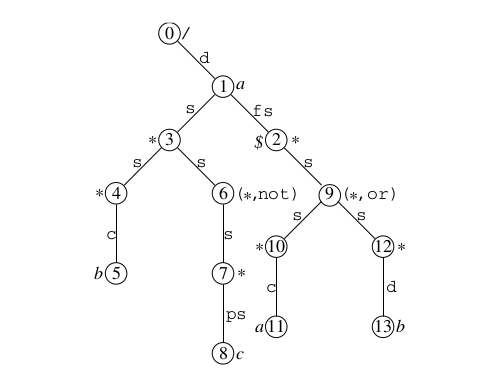
\includegraphics[scale=.5]{querytree.png}
\caption{Albero della query Q}
\end{figure}
Partendo da una query CXPath o un suo sottoinsieme è possibile costruire un albero Q della query; in figura è mostrato l'albero che corrisponde alla query 
\texttt{Q = /d::$a$[c::$b$ and not ps::$c$]/fs::*[c::$a$ or d::$b$]} dove con d si intende l'asse descendant::, con c l'asse child, con ps l'asse preceding-sibling, con fs l'asse following-sibling.\\
Nell'albero della query ogni nodo ha un etichetta con il tipo e l'eventuale operatore \texttt{bool}. A ogni arco è associato un asse.\\
Per prima cosa si costruisce un percorso lineare, detto trunk(Q) ignorando tutti i predicati dalla query.  ogni vertice di trunk(Q) corrisponde a un location step della query. L'ultimo nodo è contrassegnato con \$ è corrisponde al nodo di output della query.\\
I predicati possono essere ora aggiunti in maniera ricorsiva aggiungendo un arco con asse \texttt{self::} collegato al sotto albero del predicato; questo sottoalbero ha come radice un nodo di tipo * con l'eventuale operazione booleana (\texttt{and} può essere sottointesa). Viene creato un ramo per ogni operando che viene valutato ricorsivamente.
\\\\
Ramanan dimostra due importanti risultati:
\begin{itemize}
\item Valutare un espressione di $CXPath^+$ equivale a calcolare la simulazione del grafo della query Q rispetto al grafo del documento D
\item L'indice basato sulla simulazione è il più piccolo indice in grado di coprire le query di tipo $BPQ^+$
\end{itemize}
Il secondo risultato è interessante in quanto è noto che gli indici basati su bisimulazione preservano il linguaggio delle $BPQ$ ma nel caso in cui si incontrano query che non fanno uso dell'operatore not è possibile sfruttare la riduzione spaziale offerta dagli indici basati su simulazione.


%%%%%%%%%%%%%%%%%%%%%%%%%%
%CAPITOLO 4 XML INDEXING % 
%%%%%%%%%%%%%%%%%%%%%%%%%%

\chapter{XML Indexing}
Elaborare una query XPath significa visitare il documento e restituire i nodi che rispondo alle proprietà desiderate; nella visualizzazione ad albero del DOM questo corrisponde a una visita in profondità. Per documenti molto grandi tuttavia questa visita diventa molto onerosa anche per query molto semplici. Lo scopo degli indici XML è quello di semplificare l'operazione riducendo lo spazio e il tempo di ricerca in qualche modo.\\
Da un punto di vista formale Xpath è un linguaggio con una certa espressività in grado di distinguere tutti gli elementi di un documento ma una query molto spesso non utilizza a pieno tutto il potere espressivo a disposizione. Avremo allora delle classi di query per le quali alcuni nodi saranno indistinguibili. Un indice non è altro che una struttura dati in cui i nodi non distinguibili vengono accorpati, fornendo così una struttura dati semplificata su cui valutare le query. Va notato che a volte può essere utile utilizzare un indice anche se la risposta alla query risulterà non accurata (avremo dei "falsi positivi") per poi effettuare un filtraggio dei risultati.\\\\
In questa sezione vedremo alcuni tipi di indici strutturali per documenti XML basati sui nodi e sui grafi.
\section{Indici Basati sui Nodi}
Inteval e Path Labeling sono techiche di indicizzazione basate sui nodi. Immagazzinando dei valori che riflettono in qualche modo la posizione dei nodi nella struttura dell'albero XML di trovare, dato un nodo, il nodo padre, i figli, i fratelli, i discendenti e gli antenati. Mostriamo due varianti dette \emph{Interval(o Region) Labeling} e \emph{il Prefix(o Path) Labeling} che differiscono nel etichettamento.

\subsection{Interval Labeling}
Inteval Labeling significa etichettare i nodi con un intervallo in base alla posizione nell'albero o nel documento. Esempi di questo metodo sono la tecnica \emph{(Pre,Post)} e la tecnica \emph{(Beg,End)} che vedremo in dettaglio.
\\
Nel metodo \emph{(Pre,Post)} visitiamo l'albero XML con un algoritmo di visita Pre-Order e Post-Order. Ogni volta che incontriamo un nodo lo numeriamo con la posizione di visita. Confrontando le etichette possiamo ricostruire la posizione di ogni nodo nell'albero senza mantenere la struttura dati in memoria.
\\
Nel metodo \emph{(Beg,End)} scorriamo il documento XML in maniera sequenziale mantenendo un contatore che viene incrementato ogni qual volta incontriamo un tag, un attributo, o i valori a essi associati. Assegniamo il valore del contatore all'etichetta \emph{Beg} dell'elemento quando lo incontriamo e quando giungiamo alla terminazione di questo assegniamo il valore del contatore a \emph{End}.
\\\\
\begin{example}
\begin{figure}[h]
\centering
\subfloat[]{
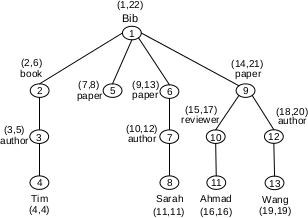
\includegraphics[scale=.7]{begend1}
}
\subfloat[]{
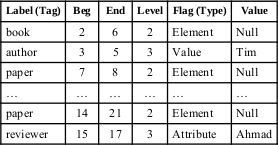
\includegraphics[scale=.7]{begend2}
}
\caption{esempio di labeling (beg,end)}
\end{figure}
\end{example}
\\
Aggiungendo una terza etichetta \emph{Level} che indica la profondità nell'albero possiamo formulare due regole per calcolare le relazioni successore-discendente e padre-figlio:
\begin{itemize}
\item \textbf{Proprietà 1:} in un albero un nodo $x$ è antenato di un nodo $y$ sse $x.Beg < y.Beg < x.End$
\item \textbf{Proprietà 2:} in un albero un nodo $x$ è padre di un nodo $y$ sse $x.Beg < y.Beg < x.End$ and $y.Level = x.Level + 1$
\end{itemize}

\subsection{Path Labeling}
Questa tecnica si basa sull'etichettare ogni nodo con un vettore in cui è indicato il percorso fino ad esso. Come esempio di questa tecnica illustreremo il metodo Dewey.
\\
Il metodo Dewey prevede che ogni etichetta rappresenti la posizione del nodo includendo come prefisso la codifica dei suoi antenati (coordinata verticale) e aggiungendo il numero del nodo tra i suoi fratelli (coordinata orizzontale). Il livello è implicitamente definito dalla lunghezza del vettore.
Per stabilire le relazioni tra due nodi sarà sufficiente effettuare un controllo di pattern matching tra le etichette.
\\
Gli antenati di un certo nodo x saranno tutti quelli la cui etichetta è una sotto-stringa dell'etichetta di x, il padre sarà il nodo la cui etichetta è soltanto un carattere più breve; ad esempio è facile verificare che il nodo $(0.3)$ è antenato del nodo $(0.3.1.0)$ e padre di $(0.3.1)$.
\\
I fratelli invece avranno un etichetta della stessa lunghezza che differirà soltanto per l'ultimo carattere; ad esempio $(0.3.1)$ e $(0.3.2)$.
\\
Il punto di forza di questo sistema è la semplicità nella verifica delle relazione e nell'aggiornamento della struttura; la grande debolezza invece la lunghezza delle etichette cresce con l'aumentare delle profondità e con essa lo spazio necessario ad immagazzinare le informazioni e il tempo necessario a calcolare le relazioni tra i nodi.
\section{Strong DataGuide}
Proposto nel 1997 da Goldman e Widom, è uno dei primi algoritmi utilizzati per il calcolo degli indici. Partendo da un grafo $G_1$, Strong DataGuide restituisce un grafo $G_2$ in cui i nodi vengono partizionati in base al percorso dalla radice al nodo. Pensando il grafo di partenza come un automa a stati finiti \textbf{non-deterministico} l'algoritmo genera il grafo dell'automa a stati finiti \textbf{deterministico} corrispondente.\\
Un indice Strong DataGuide deve soddisfare le seguenti caratteristiche di base:
\begin{itemize}
\item Ogni cammino distinto radice-nodo nel grafo di partenza compare soltanto una volta nell'indice.
\item Ogni singolo cammino nel grafo indice deve avere almeno una corrispondenza nel grafo originale, ossia non ci sono percorsi non validi nell'indice.
\end{itemize}
Essere deterministico è contemporaneamente un vantaggio e uno svantaggio in quanto i nodi con più di un padre(idref) verranno duplicati. Se consideriamo un documento con idref modellato quindi come un DAG esiste la possibilità che la cardinalità dell'indice sia maggiore di quella del grafo di partenza, vanificando lo scopo dello stesso. Nel caso invece di un documento modellato come un albero nel caso peggiore la cardinalità dell'indice sarà uguale a quella del documento.\\\\
DataGuide è in grado di fornire risposte precise e complete alle cosìdette path-query, cioè quelle query che presentano sono relazioni padre-figlio o antenato-discendente. Nel caso di query che coinvolgono anche i predicati (twig-query) la risposta ottenuta sarà completa ma non precisa e otterremo dei falsi positivi.\\\\
\begin{example}
\begin{figure}[H]
\centering
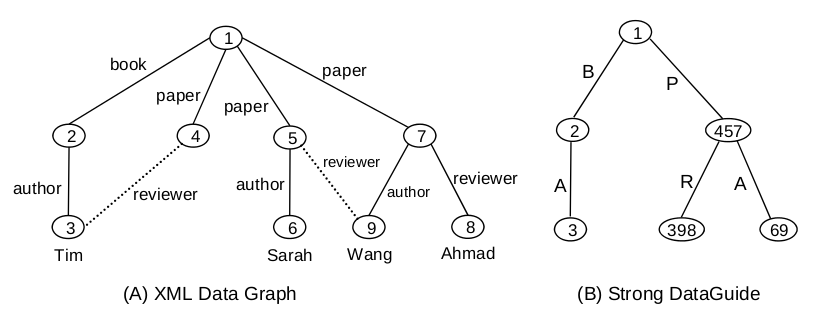
\includegraphics[scale=.5]{dataguide}
\end{figure}
\end{example}
\section{Indici Basati sulla Bisimulazione}
Vediamo due tipi di indici basati sulla simulazione: A(1)-index, in grado di coprire Path Queries, e F\&B-index, in grado di coprire anche le Twig Queries.
Entrambi questi indici risultano poco efficienti nel caso in cui i dati siano molto grandi e irregolari per via dei requisiti stringenti della relazione di bisimulazione
\subsection{1-index}
Introdotto nell 1999 da Milo e Suciu questo indice è basato sulla relazione di Bisimulazione all'indietro (Backward Bisimiluation), questa relazione è uguale alla bisimulazione vista in precedenza con la differenza che conserva gli archi entranti invece di quelli uscenti. Di seguito una definizione formale.
\begin{definition}[Backward Bisimulation]
Dati due vertici $u$ e $v$, $u \simeq v$ se:
\begin{itemize}
\item $\langle\langle u \rangle\rangle = \langle\langle v \rangle\rangle$
\item $\forall u' \in pre(u) \exists v' \in pre(v) | u' \simeq v'$
\item $\forall v' \in pre(v) \exists u' \in pre(u) | v' \simeq u'$
\end{itemize}
Diremo quindi che $u$ B-bisimula $v$; se $u \simeq v$ e $v \simeq u$ allora si ha una relazione di equivalenza che chiameremo \emph{backward-bisimulazione} $\approx^B$.
\end{definition}
1-index non è altro che il partizionamento del grafo di un documento XML secondo le classi di equivalenza della relazione di B-Bisimulazione. Per ottenere l'indice si può procedere invertendo gli archi del grafo e utilizzando un algoritmo che applica la definizione di F-bisimulazione vista nel capitolo introduttivo.\\\\
Esistono anche delle versioni approssimate dell'algoritmo 1-index, dette A(k)-Index e D(k)-index. A(k)-index calcola la bisimulazione su percorsi entranti di lunghezza k, con k impostato manualmente, invece che fino alla radice, diminuendo la precisione ma aumentando la riduzione dello spazio.D(k)-index opera alla stessa maniera ma il valore di k viene impostato dinamicamente.\\\\
\begin{example}
\begin{figure}[H]
\centering
\subfloat{
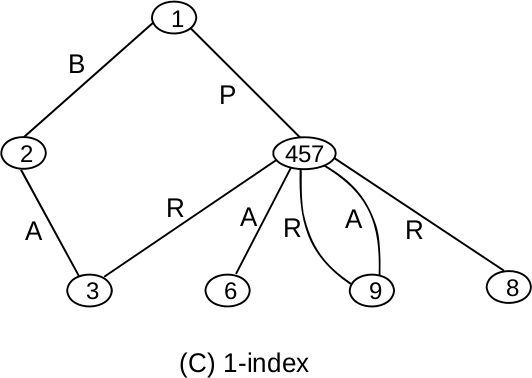
\includegraphics[scale=.3]{1-index.png}
}
\subfloat{
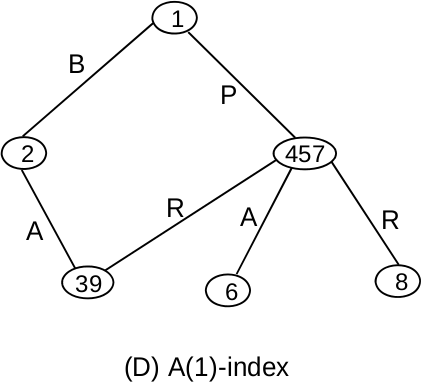
\includegraphics[scale=.3]{a1-index.png}
}
\subfloat{
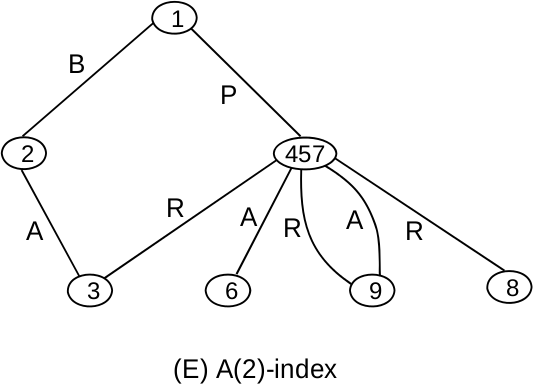
\includegraphics[scale=.3]{a2-index.png}
}
\end{figure}
\end{example}
\subsection{F\&B-index}
Sviluppato nel 2002 da Abiteboul, Buneman, et al. F\&B-index (Forward \& Backward Index) è un indice basato su bisimulazione in avanti e in indietro.\\
Questa relazione è l'unione delle condizione di Forward-simulation e Backward-simulation e permette di conservare i tipi e i gli archi sia entranti che uscenti.\\
A differenza degli indici visti in precedenza questo tipo indice è in grado di rispondere accuratamente anche a query ramificate. Kaushik, Bohannon, Naughton, e Korth (2002) hanno dimostrato che F\&B-index è l'indice più piccolo in grado di coprire le Branching Path Queries. Questo guadagno in versatilità viene però a discapito delle dimensioni dell'indice che sarà più grande per via della relazione d'equivalenza più esclusiva.
\\\\
Come per gli indici basati su B-bisimulazione anche per questo indice sono state proposte varianti approssimate, in particolare (F\&B)$^{k}$-index dove k è il parametro che gestisce l'approssimazione,e quindi le dimensioni, dell'indice in maniera affine a A(k)-index. Un altra variante dell'indice è pensata per distribuire i risultati su disco in modo da non riempire la memoria centrale, consentendo così di lavorare con documenti più grandi.\\\\
\begin{example}
\begin{figure}[H]
\centering
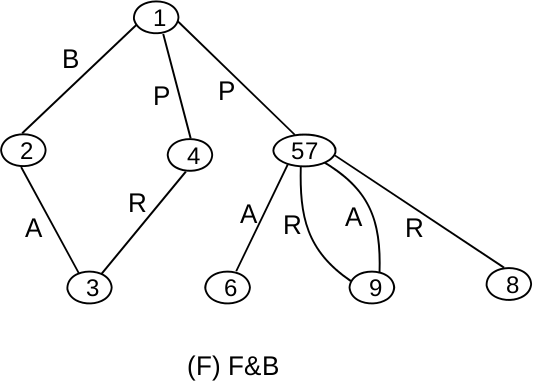
\includegraphics[scale=.4]{fb-index.png}
\end{figure}
\end{example}

\section{Indici Basati sulla Simulazione}

%%%%%%%%%%%%%%%%%%%%%%%%%%%%%
%CAPITOLO 5 IMPLEMENTAZIONE %
%%%%%%%%%%%%%%%%%%%%%%%%%%%%%

\chapter{Implementazione}

\end{document}